\subsection{Objective-conditioned open structural exploration}
\label{sec:objective-structure-v8}

The next experiment changes the design object rather than the population or
replication scale. Two fixed illustrative LossSpecs condition otherwise identical
interfaces: throughput $L_{\mathrm{count}}=-A$ and net reviewed utility
$L_{\mathrm{utility}}=3.25A-Q+0.05R$, where $A$ counts native accepted decisions,
$Q$ sums the within-decision means of actual raw reviewer scores over accepted
decisions, and $R$ counts all review records. Neither objective is a validated
measure of scientific value; an institution-written final score cannot create
$Q$. No undeclared quality, participation or fairness veto is introduced.

Each arm has two external source-generation rounds and two conditional-IID
design draws per round, for at most eight physical original-native worlds.
The five original authoring researchers, fixed local Qwen3:8B weights, two-year
horizon, four-year corpus and development seed42 remain fixed. Every candidate
is a fresh reset world with its own response journal. The study changes
objectives, not optimizer settings; it does not compare optimizers or use
held-out seeds. The initial developer graph is a design seed, not an additional
evaluated baseline with an invented score.

The designer authors arbitrary sandboxed Python, intermediate protocols,
node additions/removals, explicit connections and activity processes. No tensor
mechanism identifier is mandatory. Original researchers and native research,
project, paper, retrieval and resource state remain the forward environment;
institutional review, selection or funding may be replaced or omitted when
the explicit downstream contracts are executable. Thus containing the legacy
world does not mean requiring every legacy institution. Optional policy-free
graph-edit helpers lower complete authored transactions into the same generic
patch format; they do not complete missing semantic connections or supply a
catalogue of institutional algorithms.

Each generation receives only its own arm's objective, actual preceding
observations, source, failures, incumbent and distribution updates. The
external Codex designer identity is self-reported, not authenticated or Qwen
authorship. Conditional categorical/Gaussian score updates and declared
black-box designer-selection heuristics use actual native costs. They do not
differentiate source synthesis or researcher text. Identity proposals, repeated
IID choices and a failure to improve are legal; structural novelty is not
rewarded or required by a merit filter.

The independent read-only analysis reconstructs complete generation/authoring
history, remeasures eight native diagnostics, cross-scores every completed
world under both frozen losses and retains all failures with null loss. A
comparison metric may be unavailable without invalidating an available own-arm
loss. Each arm selects only by its own observed loss; all exact ties are
reported, with the earliest used solely as a display representative. Cross-scores
reuse development worlds, not new replications. Structural accounting compares
each system to the initial graph and its actual generation parent, separately
recording node/edge/protocol/schedule changes, literal source-body changes and
same-source renaming. A renamed node or changed initial state is not evidence
of a new algorithm or a beneficial institution.

\paragraph{Preserved pre-inference authoring failure.}
The first attempt rejects both initial definitions before any native world or
researcher response: a JavaScript JSON roundtrip changes integral floats to
integers, binding the author's patch to a normalized parent rather than the
exact saved request. The compiler correctly fails closed. Both consumed
definitions, null generation errors and unanswered next requests are preserved;
this is an aborted attempt, not a completed budget. A separately preregistered
second output uses the same correct source pin and an exact-file Python
validation workflow. Its actual-world cap remains eight across both attempts;
no unsuccessful native trajectory is replaced. The author's earlier validation
claim is explicitly corrected, not used as evidence.

\IfFileExists{generated/native-v8/results.tex}{%
  % Auto-generated from independently audited v8 evidence e932c88a73fe7fa9e3b70b487d798a1504994e3ae6841c26ff335070cbb2ffff.
% Prepared fragment only: paper integration remains an explicit reviewed action.
\begin{figure*}[t]
  \centering
  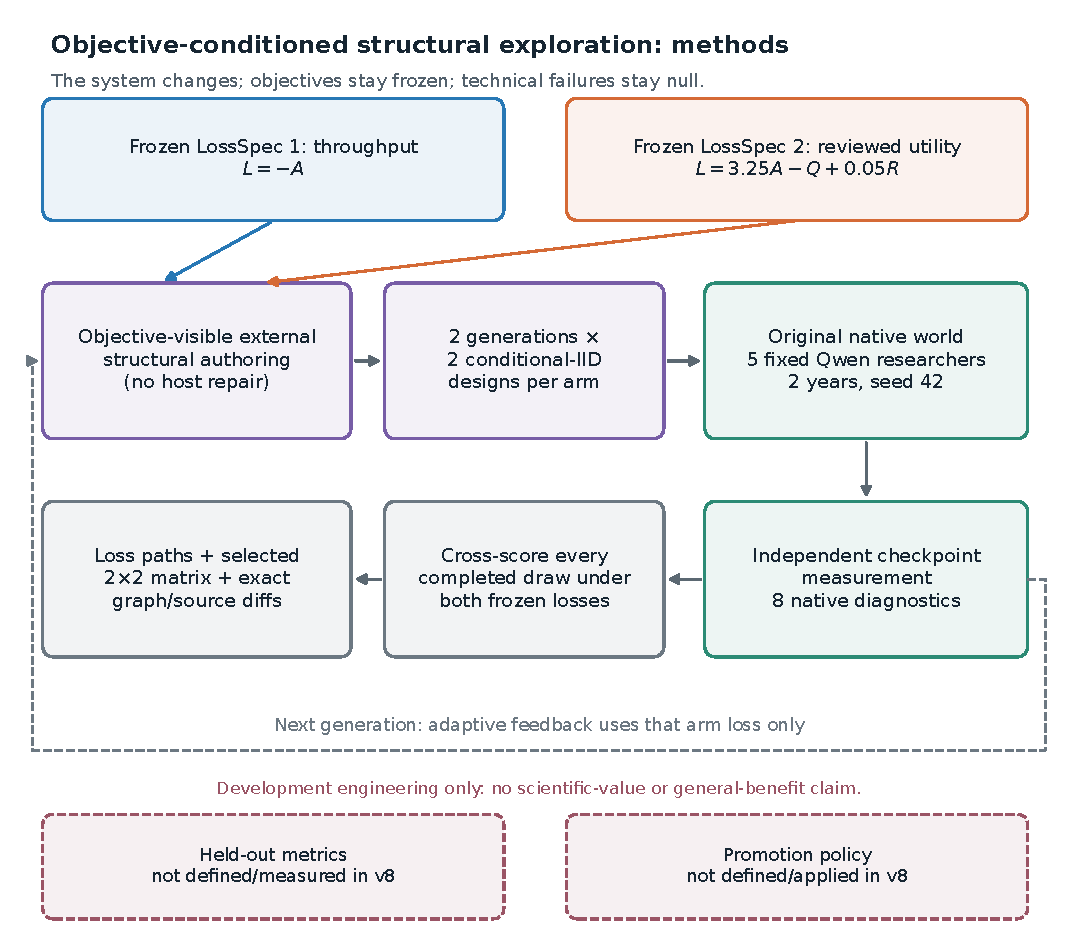
\includegraphics[width=\textwidth]{figures/native-objective-structure-v8-methods.pdf}
  \caption{Preregistered two-objective native structural exploration. The system is optimized while each LossSpec remains frozen. Held-out metrics and promotion are outside this development-engineering pilot.}
  \label{fig:native-objective-structure-v8-methods}
\end{figure*}

\begin{figure*}[t]
  \centering
  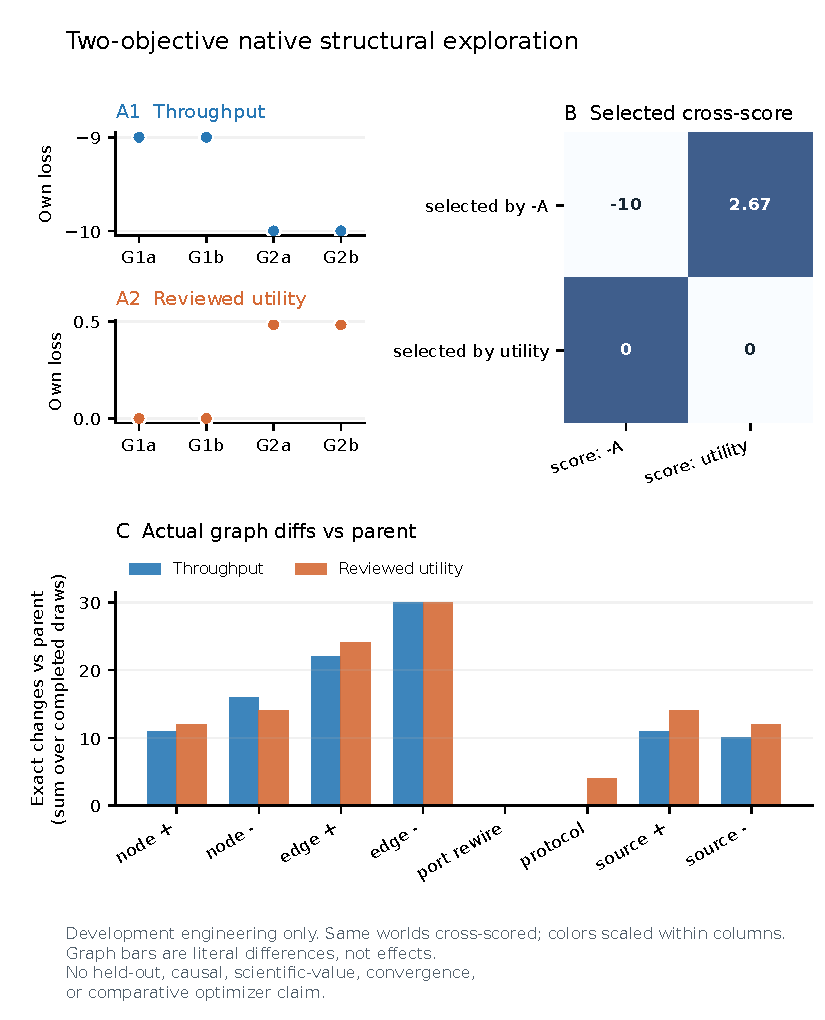
\includegraphics[width=\textwidth]{figures/native-objective-structure-v8.pdf}
  \caption{Audited development loss paths, cross-objective scores of the two selected representatives, and literal graph/source differences. Cross-scores reuse the same worlds and are not independent replications.}
  \label{fig:native-objective-structure-v8-results}
\end{figure*}

\begin{table}[t]
\centering
\caption{Selected-system development cross-scores (lower is better within a column; objectives have different units).}
\label{tab:native-objective-structure-v8-crossscores}
\begin{tabular}{lrr}
\toprule
Selection objective & $-A$ & $3.25A-Q+0.05R$ \\
\midrule
$-A$ & -10 & 2.667 \\
Reviewed utility & 0 & 0 \\
\bottomrule
\end{tabular}
\end{table}

\paragraph{Scope.} These are objective-conditioned development-engineering observations. Observed loss changes do not establish held-out, causal, scientific-value, optimizer-convergence, or generalized institutional benefit. Technical failures remain null rather than numerical penalties.
%
}{%
  \paragraph{Execution status.} The preregistered actual-native exploration is
  in progress. No completed v8 structural comparison, held-out benefit or
  scientific institutional discovery is claimed here.%
}
